\documentclass[twoside,10pt,a4paper]{article}
\usepackage[utf8]{inputenc}
\usepackage[english]{babel}
\usepackage{amsmath}
\usepackage{amsfonts}
\usepackage{amssymb}
\usepackage{graphicx}

\usepackage[left=2cm,right=2cm,top=2cm,bottom=3cm]{geometry}
\usepackage{fancyvrb}
\usepackage{listings}
\usepackage{xparse}
\usepackage{tikz} % ajout de dessins LaTeX
\usepackage{graphicx}
\usepackage{float}  % alignement des figures
\usepackage{fancyhdr}
\usepackage{enumitem}
\usepackage{verbatim}
\usepackage{xcolor}
\usepackage{cancel}

\usepackage{caption}
\usepackage{subcaption}

\pagestyle{fancy} %fancyhdr
	\fancyhf{} %fancyhdr
	\renewcommand{\sectionmark}[1]{\markboth{#1}{}}
	\fancyhead[R]{NLDCI Set 5 Solutions} %INSERT TITLE HERE FOR fancyhdr
	\fancyhead[L]{\nouppercase{\leftmark}} %fancyhdr
	\cfoot{\thepage} %fancyhdr
	\setlength{\headheight}{35pt}
	\setlength{\parindent}{0pt}
	
	\definecolor{MyBlue}{HTML}{4A90E2}
	\definecolor{MyRed}{HTML}{D0021B}
	\definecolor{MyGreen}{HTML}{7ED321} % Same color use in Mathcha

\begin{titlepage}
\title{\huge \textbf{Nonlinear Dynamics \& Chaos I \\ \Large Exercice Set 5 Solutions}}	%TITLE
\author{ }		%AUTHOR
\date{ }	%DATE

\end{titlepage}


\begin{document}

\maketitle

\section*{Question 1}
Consider the quadratic \textit{Duffing equation}
\begin{align*}
	\dot{u} &= v, \\
	\dot{v} &= \beta u - u^2 - \delta v,
\end{align*}
where $\delta > 0$, and $0 \leq |\beta| \ll 1$.

\begin{enumerate}[label=(\alph*)]
	\item Construct a $\beta$-dependent center manifold up to quadratic order near the origin for small $\beta$ values.
	\item Construct a stability diagram for the reduced system on the center manifold using $\beta$ as a bifurcation parameter.
\end{enumerate}

\section*{Solution 1}
\begin{enumerate}[label=(\alph*)]
\item Linearized dynamics around fixed point $(0,0)$
\begin{equation*}
	\dot{\eta} = A\eta \; , \; A = \begin{bmatrix}
		0 & 1 \\ \beta & -\delta
	\end{bmatrix} \; , \; \text{eig}(A) = \lambda_{1,2} = -\delta \pm \sqrt{\delta^2 - \beta}
\end{equation*}
Note that $\lambda_1 = 0 \; , \; \lambda_2 = -\delta$ for $\beta = 0$. Thus, by the center manifold theorem, we have a 1-dimensional center manifold passing through the origin and a unique 1-dimensional stable manifold.


\begin{itemize}
	\item Consider the extended system
\end{itemize}

\begin{align*}
	\dot{\beta} &= 0 \\
	\begin{bmatrix}
		\dot{u} \\ \dot{v}
	\end{bmatrix}
	&= \underbrace{\begin{bmatrix}
		0 & 1 \\ 0 & -\delta
	\end{bmatrix}}_{B} \begin{bmatrix}
		u \\ v
	\end{bmatrix}
	+
	\begin{bmatrix}
		0 \\ \beta u - u^2
	\end{bmatrix}
\end{align*}

\begin{align*}
	& \text{Eigenvalues of } B: \lambda_1 = 0 \; , \; \lambda_2 = -\delta \\
	& \text{Eigenvectors of } B: e_1 = \begin{bmatrix}
		1 \\ 0
	\end{bmatrix} \; , \; e_2 = \begin{bmatrix}
		\frac{1}{\delta} \\ -1
	\end{bmatrix}
\end{align*}
From the eigenvalues and eigenvectors, we can perform a change of coordinates
\begin{equation*}
	\begin{bmatrix}
		u \\ v
	\end{bmatrix} = T \begin{bmatrix}
		x \\ y
	\end{bmatrix} \; , \; T = [e_1 \vert e_2] = \begin{bmatrix}
		1 & \frac{1}{\delta} \\ 0 & -1
	\end{bmatrix} \; , \; T^{-1} = \begin{bmatrix}
		1 & \frac{1}{\delta} \\ 0 & -1
	\end{bmatrix} = T
\end{equation*}
\begin{equation*}
	\Longrightarrow u = x + \frac{y}{\delta} \; , \; v = -y
\end{equation*}

\begin{align}
	\Longrightarrow \begin{bmatrix}
		\dot{x} \\ \dot{y}
	\end{bmatrix} &= T^{-1}BT \begin{bmatrix}
		x \\ y
	\end{bmatrix} + T^{-1} \begin{bmatrix}
		0 \\ \beta u - u^2
	\end{bmatrix} \nonumber \\
	\label{S04E021}
	&= \begin{bmatrix}
		0  & 0 \\ 0 & -\delta
	\end{bmatrix} \begin{bmatrix}
		x \\ y
	\end{bmatrix} + \begin{bmatrix}
		\frac{1}{\delta} \left( \beta \left( x + \frac{y}{\delta} \right) - \left( x + \frac{y}{\delta} \right)^2 \right) \\
		-\beta \left( x + \frac{y}{\delta} \right) + \left( x + \frac{y}{\delta} \right)^2
	\end{bmatrix} 
\end{align}

Seek center manifold as a graph over center subspace locally as

\begin{align}
	y &= h(x, \beta) = a_1x^2 + a_2x\beta + \cancel{a_3\beta^2} + \mathcal{O}(3) \nonumber \\
	\label{S04E022}
	\dot{y} &= \frac{\partial h}{\partial x}\dot{x} + \frac{\partial h}{\partial \beta} \cancelto{0}{\dot{\beta}}
\end{align}
Note: We cancel the term $a_3 \beta^2$ to respect the existence of the fixed point.

Use invariance in (\ref{S04E022}): 
\begin{align}
	\label{S04E023}	
	\Longrightarrow \dot{y} &= (2a_1x + a_2 \beta) \left[ \frac{1}{\delta} \left( \beta \left( x + \frac{h(x,\beta)}{\delta} \right) - \left( x + \frac{h(x,\beta)}{\delta} \right)^2 \right) \right] \\
	\label{S04E024}	
	\text{But also } \dot{y} &= -\delta h(x, \beta) - \beta \left( x + \frac{h(x,\beta)}{\delta} \right) + \left( x + \frac{h(x, \beta)}{\delta} \right)^2
\end{align}
Comparing $\mathcal{O}(2)$ terms in (\ref{S04E023}) \& (\ref{S04E024}), we get:
\begin{align*}
	x^2: \qquad -\delta a_1 + 1 = 0 &\Longrightarrow a_1 = \frac{1}{\delta} \\
	x\beta: \qquad -\delta a_2 - 1 = 0 &\Longrightarrow -a_2 = \frac{1}{\delta}
\end{align*}
Thus, the $\beta$-dependent center manifold is given by
\begin{equation} \label{S04E025}
	h(x, \beta) = \frac{x^2}{\delta} - \frac{x \beta}{\delta} + \mathcal{O}(3)
\end{equation} 
Substitute (\ref{S04E025}) into first equation in (\ref{S04E021}) to obtain reduced dynamics on the center manifold: $W^C_\beta (0)$ up to quadratic order.
\begin{align*}
	\dot{x} &= \frac{1}{\delta} \left[ \beta \left( x + \frac{h(x, \beta)}{\delta} \right) - \left( x + \frac{h(x, \beta)}{\delta} \right)^2 \right] \\
	&= \frac{1}{\delta} [\beta x - x^2] + \mathcal{O}(3)
\end{align*}

\item 
\begin{equation*}
	\dot{x} = \frac{1}{\delta} [\beta x - x^2]
\end{equation*}
Fixed points:
\begin{align*}
	x &= 0, \\
	\beta &= x
\end{align*}

\newpage

\begin{figure}[H]
	\centering
	
\includegraphics[scale=0.9]{Graphics/S01D01.pdf}
	\caption{Transcritical bifurcation}
\end{figure}

\end{enumerate}

\newpage

\section*{Question 2}
Consider a dynamical system that has a pair of purely imaginary eigenvalues at its fixed point for the parameter value $\mu=0$. As we have seen, a linear change of coordinates and a center manifold reduction gives the two-dimensional reduced dynamical system


\begin{align}
\label{1}
\dot{x} &= \delta(\mu)x - \omega(\mu)y + f(x, y, \mu), \\
\dot{y} &= \delta(\mu)y+\omega(\mu)x + g(x,y,\mu),
\end{align}
where $\delta(\mu)=\text{Re }\lambda(\mu)$, $\omega(\mu) = \text{Im }\lambda(\mu)$. (Here $\lambda(\mu)$ and $\bar{\lambda(\mu)}$ is the pair of complex eigenvalues that crosses the imaginary axis at $\mu=0$.)

Recall that in polar coordinates, the truncated normal form of \eqref{1} can be written as

\begin{align*}
\dot{r} &= r(d_0\mu + a_0 r^2), \\
\dot{\theta} &= \omega_0 + b_0\mu + c_0r^2,
\end{align*}

where

\begin{align*}
d_0 &= \delta'(0), \quad \omega_0 = \omega(0) \\
a_0 &= \frac{1}{16}\left[f_{xxx}+f_{xyy}+g_{xxy}+g_{yyy} \right]_{x=y=0,\mu=0} \\
	&+ \frac{1}{16\omega_0}\left[f_{xy}(f_{xx}+f_{yy}) - g_{xy}(g_{xx} + g_{yy}) - f_{xx}g_{xx}+f_{yy}g_{yy} \right]_{x=y=0, \mu=0}.
\end{align*}

These classic formulae are used in all applications where Hopf bifurcations are analyzed.

As an application of these results, consider now the stick-slip oscillator

\begin{equation*}
m\ddot{x}+c\dot{x}+kx=F_f, \qquad F_f=mg\mu_0\left(1+e^{-\beta |v_0-\dot{x}|} \right)\text{sign }(v_0-\dot{x}),
\end{equation*}

where $m$ is the mass of the oscillator, $g$ is the constant of gravity, $\beta>0$ is a constant, $\mu_0$ is the Coulomb (static) friction coefficient, $v_0$ is the speed of the belt, $x$ is the position of the mass on the belt, $c$ is the coefficient of viscous damping, and $k$ is the spring coefficient (see Fig. \ref{fig2}).

\begin{figure}[h!]
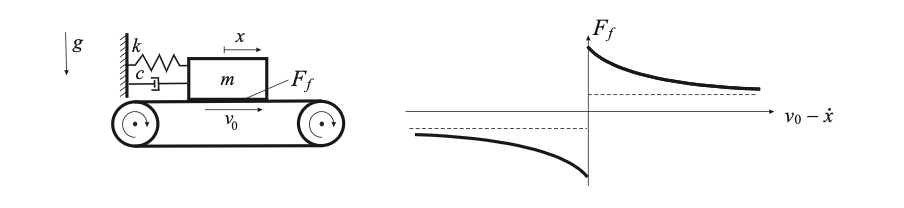
\includegraphics[width = \textwidth]{Graphics/hopf.png}
\caption{Stick-slip oscillator and its dry-friction force as a function of the relative velocity between the mass and the belt.}
\label{fig2}
\end{figure}
\begin{enumerate}[label=(\alph*)]
\item Find a condition under which the system has an asymptotically stable fixed point.
\item Show that a subcritical Hopf bifurcation takes place when the above condition is violated. (Use $v_0$ as a bifurcation parameter.)
\item Calculate the approximate amplitude of the bifurcating limit cycle.
%\item Pick parameter values for which a stable limit cycle coexists with the stable equilibrium (close to the bifurcation point, i.e., for $v_0>0$ small). For these parameter values, plot trajectories in the phase space to illustrate the two competing stable behaviors. Also plot the limit cycle amplitude you obtained from your normal form calculation, and compare your numerical and analytical results. 
\end{enumerate}
\section*{Solution 2}
\subsection*{(a)}
Let $x_1=x$ and $x_2=\dot{x}$. Then the system can be written as
\begin{align*}
\dot{x}_1&=x_2\\
\dot{x}_2&=-\frac{k}{m}x_1 -\frac{c}{m}x_2 +\frac{1}{m}F_f(x_2).
\end{align*}

The fixed point is at 
$$
x^{0}_1=\frac{1}{k}F_f(0)=\frac{mg\mu_0}{k}\left(1+e^{-\beta|v_0|} \right)\text{sign }(v_0), \quad x^{0}_2=0.
$$

Let us now shift the origin to the fixed point by introducing new coordinates as $z_1 = x_1 - x^0_1$ and $z_2=x_2$. 
Then 
\begin{align}
\label{eq111}
\dot{z}_1&=z_2\\
\dot{z}_2&=-\frac{k}{m}z_1 -\frac{c}{m}z_2 +\frac{1}{m}F_f(z_2)-\frac{1}{m}F_f(0),
\end{align}
with the fixed point at $z_1=z_2=0$. The linearized system is given by
\begin{equation}
\dot{\xi}=\begin{pmatrix} 0 & 1 \\ -\frac{k}{m} & \mu \end{pmatrix}\xi, 
\end{equation}
where we have introduced the parameter
\begin{equation}
\boxed{\mu=\frac{1}{m}\left(F_f'(0)-c\right) = g\beta \mu_0 e^{-\beta|v_0|}-\frac{c}{m}}. 
\end{equation}
The eigenvalues of the coefficient matrix are 

\begin{equation}
\label{eq12}
\lambda_{1,2} = \frac{\mu}{2}\pm \frac{1}{2}\sqrt{\mu^2-\frac{4k}{m}}.
\end{equation}
For the remainder of the discussion, let us assume that  $|\mu|$ is not too big; specifically $\mu^2 < \frac{4k}{m}$. This is in line with our previous assumption to treat $\mu$ as a bifurcation parameter. In this case, the real part of $\lambda_{1,2}$ can simply be read off from \eqref{eq12} as 

$$
\text{Re }(\lambda_{1,2}) = \frac{\mu}{2}. 
$$

As a result, if $\mu<0$ then Re $(\lambda_1)<0$ and Re $(\lambda_2)<0$, hence the fixed point is \underline{asymptotically stable} by the Hartman-Grobman theorem. This condition translates into
$$
\mu<0 \Leftrightarrow g\beta\mu_0e^{-\beta|v_0|}<\frac{c}{m} \Leftrightarrow |v_0| > \frac{1}{\beta}\log\left(\frac{mg\beta \mu_0}{c} \right).
$$
Hence, if \begin{equation}
\label{eqcond}
|v_0| > \frac{1}{\beta}\log\left(\frac{mg\beta \mu_0}{c} \right),
\end{equation}
then $(z_1=z_2=0)$ is an asymptotically stable fixed point. 

\subsubsection*{Remark}
Note that if the viscous damping $c$ is large enough such that $c>mg\beta \mu_0$ then $\log\left(\frac{mg\beta \mu_0}{c} \right)<0$. Then the condition \eqref{eqcond} is satisfied for any $v_0\neq 0$ and ($z_1=z_2=0$) is asymptotically stable for any $v_0$.
\subsection*{(b)}
For $0<\mu \ll 1$ we have Re $(\lambda_{1,2})>0$. At $\mu=0$ the eigenvalues cross the imaginary axis at 
$$
\lambda_{1,2}(\mu=0)=\pm i \sqrt{\frac{4k}{m}}.
$$
Now let $-1\ll\mu< 0$. Then the eigenvalues are 
$$
\lambda_{1,2}=\frac{\mu}{2}\pm i\frac{1}{2} \sqrt{\frac{4k}{m}-\mu^2}.
$$

Define 
\begin{equation}
\label{eq14}
\boxed{\delta(\mu)=\frac{\mu}{2}, \quad \omega(\mu)=\frac{1}{2}\sqrt{\frac{4k}{m}-\mu^2}.}
\end{equation}
Then, we can separate the linear and nonlinear terms from the system \eqref{eq111} and write it as
\begin{equation}
\label{transf}
\begin{pmatrix} \dot{z}_1 \\ \dot{z}_2 \end{pmatrix} = A\begin{pmatrix} z_1 \\ z_2 \end{pmatrix} + \begin{pmatrix} 0 \\ \frac{1}{m}F_f(z_2)-\frac{1}{m}F'_f(0)z_2 - \frac{1}{m}F_f(0)\end{pmatrix},
\end{equation}
where we have denoted the linear part as $$A=\begin{pmatrix} 0 & 1 \\ -\frac{k}{m} & \mu \end{pmatrix}.$$ The eigenvalues of $A$ are $\delta(\mu)\pm i \omega(\mu)$. To simplify the calculation of the eigenvectors, we note that  (as a consequence of \eqref{eq14})

$$
\mu = 2\delta \quad \frac{k}{m} = \delta^2 + \mu^2
$$

and hence
$$
A=\begin{pmatrix}0 & 1 \\ -\delta^2 -\omega^2 & 2\delta  \end{pmatrix}.
$$

We then search for a vector $s$ such that 

$$
As-(\delta + i\omega)s =\begin{pmatrix}-\delta - i\omega & 1 \\ -\delta^2 -\omega^2 & \delta-i\omega  \end{pmatrix}   \begin{pmatrix} s_1 \\ s_2\end{pmatrix}.
$$

For example, the non-normalized vector

$$
s = \begin{pmatrix} 1  \\ \delta + i\omega \end{pmatrix}
$$
is a good choice. To separate the real and imaginary parts of the eigenvector we write it as 
$$
s= \begin{pmatrix} 1\\ \delta(\mu) \end{pmatrix}\pm i \begin{pmatrix} 0 \\ \omega(\mu) \end{pmatrix}.
$$

Selecting the real and imaginary parts of $s$ as basis vectors then puts $A$ in the desired block-diagonal form,  that is 
$$
A=VDV^{-1},
$$
where $$
D=\begin{pmatrix} \delta & \omega \\ -\omega & \delta \end{pmatrix} \text{ and } V=\begin{pmatrix} 1 & 0 \\ \delta & \omega  \end{pmatrix}.
$$
This means, that under  the change of variables 
$$
\begin{pmatrix} z_1 \\ z_2 \end{pmatrix} = V \begin{pmatrix} u \\ v\end{pmatrix}
$$
 we get the transformed dynamical system
 
 \begin{equation}
 \begin{pmatrix} \dot{u} \\ \dot{v} \end{pmatrix} = \begin{pmatrix} \delta  & \omega  \\  -\omega & \delta \end{pmatrix}\begin{pmatrix} u \\ v  \end{pmatrix} + \frac{1}{m\omega}\begin{pmatrix} 0  \\ F_f(\delta u + \omega v) - F'_f(0)(\delta u + \omega v) - F_f (0)\end{pmatrix}.
 \end{equation}
 This is the desired form for the dynamical system defined in the problem description. Note that we may put
 \begin{align*}
 f(x,y,\mu) &=0 \\
 g(x,y,\mu) &= \frac{1}{m\omega} F_f(\delta u + \omega v) - F'_f(0)(\delta u + \omega v) - F_f (0)
 \end{align*}
 to compute the desired parameters
 
$$
d_0 = \delta'(0)=\frac{1}{2}, \quad \omega_0 = \omega(0)= \sqrt{\frac{k}{m}}, \quad a_0 = \frac{kg\mu_0 \beta^3 e^{-\beta |v_0|}}{16m},
$$
where we have used that 
$$ 
g_{vvv}(0,0,0) = \frac{k}{m^2}F'''(0)= \frac{kg\mu_0 \beta^3 e^{-\beta |v_0|}}{m}.
$$

According to the Hopf-Bogdanov theorem, the radial component of the normal form of the dynamics can be written as
\begin{equation}
\boxed{\dot{r}=r\left( \frac{\mu}{2}+ \frac{kg\mu_0 \beta^3 e^{-\beta |v_0|}}{16m}r^2\right)},
\end{equation}
which has fixed points 
$$
r=0 \text{ which corresponds to the stable fixed point}
$$
$$
r = \pm \sqrt{\frac{-8\mu m e^{\beta |v_0|}}{kg\mu_0 \beta^3}}, \text{ which corresponds to the unstable limit cycle. }
$$
Expressed as a function of $v_0$, the bifurcation occurs at 
$$
v_C = \frac{1}{\beta}\log \left(\frac{mg\beta \mu_0}{c} \right).
$$

\subsubsection*{(c)} For $\mu<0$ the amplitude of the unstable limit cycle is 

$$
r_0 = \sqrt{\frac{-8\mu m e^{\beta |v_0|}}{kg\mu_0 \beta^3}}
$$
\end{document}